Interfata de administrare reprezinta ansablul de componente software prin intermediul careia operatorii RODA intervin in functionarea sistemului. 

\section{Tehnologie}


Interfata de administrare RODA se bazeaza pe sistemul de librarii ExtJS 4.2, sistem care permite realizarea unei aplicatii web in interiorul programului de navigare pe internet. Astfel, interfata de administrare RODA functioneaza foarte asemanator cu un program nativ, chiar daca este operata cu ajutorul browserului. 

ExtJS este in acest moment una dintre cele mai puternice biblioteci pentru constructia aplicatiilor WEB complexe, cu o compatibilitate cu diferitele browsere aproape completa care contine o lista completa de componente vizuale care pot fi utilizate direct. 

ExtJS extinde modul de programare clasic Javascript, permitand constructia unui sistem de clase. Fiecare element al interfetei se obtine prin constructia unei clase proprii prin extinderea uneia dintre clasele oferite de biblioteca ExtJS. Toate clasele aplicatiei WEB sunt incluse intr-un namespace propriu care evita coliziunile. Namespace-ul modulului de administrare este RODAdmin iar numele claselor construite pentru interfata de administrare este de tipul: "RODAdmin.view.MainViewport". 
Clasele pot fi apelate prin intermediul unui alias definit in interiorul acestora cu o instructiunea: "alias: 'widget.mainviewport'". 

ExtJS ofera o serie de elemente ajutatoare la constructia claselor, una dintre ele fiind constructia automata de metode de scriere sau citire (gettere si settere) pentru toti parametrii care sunt definiti la initializarea clasei in obiectul config. 

Sistemul de clase ExtJS si arhitectura biliotecilor conduce la aplicatii care sunt distribuite intr-un numar foarte mare de fisiere javascript (fiecare clasa este de obicei definita in propriul fisier). Aceasta impartire se face de obicei pentru usurinta dezvoltarii aplicatiei si pentru claritatea codului, de obicei, in momentul in care aplicatia trece in productie aceste fisiere se combina intr-unul singur. Dar, in faza de dezvoltare ExtJS ofera un sistem de incarcare dinamica a tuturor fisierelor care sunt solicitate in definirea claselor, evitand nevoia intretinerii fisierelor complexe de bootstrap pe care alte medii de dezvoltare javascript le solicita. 

ExtJS permite (de la versiunea 4.0) impartirea claselor in mai multe tipuri, urmarind indeaproape celebrul pattern Model View Controller. Astfel, clasele care definesc componentele cu care interactioneaza utilizatorul (cele care se vad in pagina aplicatiei) sunt view-uri si sunt declarate in fisiere care se gasesc in namespace-ul “view” a aplicatiei. Clasele care definesc structura datelor care se transfera intre aplicatia client si server sunt declarate in fisiere care se gasesc in namespace-ul “model” iar cele in care se definesc actiunile pe care aplicatia trebuie sa le execute in momentul in care utilizatorul interactioneaza cu view-urile sunt definite in namespace-ul “controller”. 

Structura unei aplicatii Extjs mai poate contine si alte feluri de componente in afara de modele, view-uri si controllere. Acestea sunt prezentate pe scurt in cele ce urmeaza:

\textbf{proxy} clase care se ocupa de comunicarea cu locul in care sunt tinute datele. Exista doua feluri principale de proxy-uri, tip client si tip server. Proxy-urile tip client sunt folosite pentru stocare locala, de obicei temporara, fie in memorie, fie in sesiunea browserului daca acesta suporta. Proxy-urile de tip server sunt si ele de cateva feluri, in functie de modul de comunicare cu serverul: Ajax, REST, JsonP, Direct. RODA foloseste atat proxy de tip Ajax cat si proxy de tip REST. 
\textbf{store} clase care incapsuleaza datele primite de la server sau specificate in alte moduri (inline). In esenta, un store este o combinatie intre un model (care determina structura datelor) si un proxy (care determina provenienta datelor). Astfel, un store stie de unde sa ia datele si in ce forma sunt acestea. Multe clase de tip view se bazeaza pe clase de tip store pentru obtinerea datelor. 

ExtJS este distribuit intr-un sistem dual de licentiere, GPL pentru proiectele opensource (asa cum va fi RODA) sau comercial pentru proiectele comerciale. 

Protocolul de comunicare dintre interfata de administrare RODA si serverul principal se bazeaza pe JSON (JavaScript Object Notation) care este un format de reprezentare a datelor utilizat in mod special in javascript. 

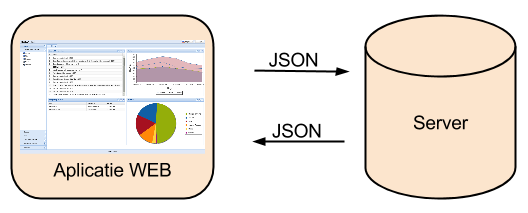
\includegraphics[width=10cm]{img/json}

JSON utilizeaza text simplu si organizeaza datele in seturi de tip eticheta - valoare. Structurile de date mai complexe se pot construi utilizand parantezele, structurile de tip lista fiind specificate prin paranteze drepte [] iar structurile de tip obiect prin paranteze acolade {}. 


\section{Componente generale ale interfetei de administrare}

\subsection{Viewport}

Exista doua moduri principale de a prezenta o aplicatie ExtJS in browser: fie afisarea ei intr-un component al unei pagini existente, fie afisarea ei in toata fereastra browserului. In cazul componentului databrowser, de exemplu, se foloseste prima varianta de prezentare pentru mentinerea catorva elemente de design (header, footer) comune cu celelalte pagini ale site-ului. In cazul interfetei de administrare, pentru ca toate scenariile de utilizare ale acesteia indica utilizarea ei exclusiva, se foloseste varianta a doua, afisarea ei in toata fereastra browserului. Aceasta se face prin includerea intregii aplicatii intr-un container special, numit viewport. 

Viewportul aplicatiei RODA este impartit in patru suprafete distincte, dintre care doua sunt importante: zona de vest in care se va incarca componentul meniu (cel care permite selectia diveritelor componente ale aplicatiei) si zona centrala, cea care acopera cea mai mare suprafata, in care se incarca containerul care va contine diferitele module de lucru alese din meniul din stanga. 

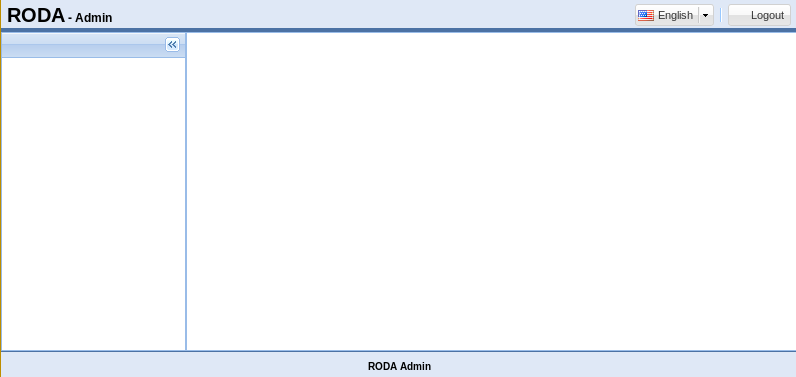
\includegraphics[width=13cm]{img/viewport}

\subsection{Sistemul de internationalizare}

Sistemul de internationalizare este un set de componente care permite schimbarea limbii interfetei de administrare. Aceste componente sunt: un view care reprezinta meniul de selectie a limbii, un controller si un set de fisiere care contin textele traduse. Controllerul reincarca fereastra browserului in momentul modificarii de limba. 

\subsection{Sistemul de linkuri interne}

Aplicatiile Web complete (ca sistemul de administrare RODA) sunt complet integrate si se incarca de la un singur URL. De aceea, in afara unor configurari speciale, ele nu permit linkuri interne, altfel spus nu este posibil ca printr-un anumit URL sa determinam aparitia unui anumit component la incarcarea aplicatiei. 

Adaugarea unui astfel de comportament (numit de multe ori “deep linking”) sau “routing” necesita constructia unui component special care sa se execute de fiecare data la incarcarea aplicatiei si sa urmareasca adaugarea diferitelor siruri de caractere la url-ul principal prin utilizarea sistemului de bookmarkuri: 

De exemplu, daca aplicatia se afla la adresa http://www.roda.ro/admin/index.html, prin apelarea url-ului: http://www.roda.ro/admin/index.html\#menu-studiesmain, aplicatia va lansa automat componentul de management al studiilor dupa incarcarea interfetei. 

Implementarea sistemului de rutare porneste de la componentul ‘Ext.util.History’. Acesta permite accesarea sistemului de istoric al browserului (cel utilizat de catre butoanele “back” si “forward”) si inregistrarea unor etichete in acesta. In acest mod e posibila urmarirea diferitelor pozitii in interiorul aplicatiei. 

Componentul pentru accesarea istoricului se initializeaza la incarcarea paginii in broeser. In cazul in care adresa solicitata are pe langa fisierul principal un bookmark, componentul ‘History’ va declansa un eveniment special pa care il va capta controllerul principal al aplicatiei. 


\subsection{Monitorul sesiunii}

Monitorul sesiunii este un component care se incarca la startul aplicatiei si urmareste ca perioada de inactivitate a interfetei sa nu depaseasca durata sesiunii de autentificare de pe server. Astfel, se evita situatiile in care sesiunea serverului expira si operatorul nu este anuntat. 

\subsection{Meniul aplicatiei}

Componentele aplicatiei disponibile operatorilor sunt accesibile prin intermediul meniului principal. Meniul principal se construieste dupa autentificare, in functie de componentele pe care utilizatorul curent are dreptul sa le acceseze. Astfel, serverul este cel care decide care elemente ale interfetei sunt disponibile pentru un anumit operator si care nu. 

Meniul aplicatiei este compus, ca majoritatea modulelor dintr-un view, un store, un model si un controller. Controllerul se activeaza in momentul incarcarii panoului principal si comanda incarcarea datelor de pe server prin intermediul store-ului atasat. Odata incarcate, controllerul adauga in meniul principal toate componentele disponibile in JSON-ul venit de la server. 


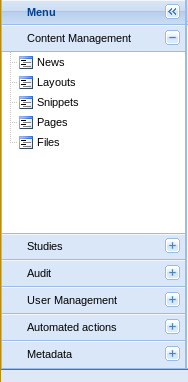
\includegraphics[width=5cm]{img/menu}

Datele care vin de la server contin intrari de meniu si sub-meniu. Fiecare intrare are un id, un text (care va fi tradus de componentul de internationalizare), o specificare a pictogramei corespunzatoare, id-ul parinte (daca este vorba de un subnod), numele clasei (daca elementul de meniu corespunde cu un modul care trebuie lansat la apelare) si specificarea leaf: true/false care informeaza store-ul ca structura arborescenta se incheie aici (leaf: true) sau are elemente subordonate (leaf: false). 

In continuare se poate vedea un fragment din raspunsul JSON:

\begin{lstlisting}[language=json,firstnumber=1]
{"items" : [ {
                "id" : "1",
                "text" : "menu_cms",
                "iconCls" : "menu_cms",
                "parent_id" : "0",
                "className" : "",
                "leaf" : false,
                "items" : [{
                            "id" : "11",
                            "text" : "cms_dashboard",
                            "iconCls" : "menu_cms_dashboard",
                            "parent_id" : "1",
                            "className" : "cmsdashboard",
                            "leaf" : true
                        },
                        {
                            "id" : "12",
                            "text" : "cms_layouts",
                            "iconCls" : "menu_cms_layout",
                            "parent_id" : "1",
                            "className" : "cmslayouts",
                            "leaf" : true
                        },
                        {
                            "id" : "13",
                            "text" : "cms_snippets",
                            "iconCls" : "menu_cms_snippet",
                            "parent_id" : "1",
                            "className" : "cmssnippets",
                            "leaf" : true
                        },
                        {
                            "id" : "14",
                            "text" : "cms_files",
                            "iconCls" : "menu_cms_files",
                            "parent_id" : "1",
                            "className" : "cmsfiles",
                            "leaf" : true
                        },
		}
	]
}

\end{lstlisting}


\subsection{Panoul de continut}

Panoul de continut este panoul principal in care se incarca componentele aplicatiei apelate din panoul de meniu. Panoul de continut permite incarcarea mai multor componente simultan, in taburi diferite. Fiecare component se poate incarca o singura data, astfel, submodulul de administrare a paginilor din modulul cms va fi prezent o singura data in panoul de continut. 

Componentele se incarca in panoul de continut in doua moduri: fie prin apelarea lor din meniu, prin intermediul controllerului ‘Menu’, fie prin apelarea lor din controllerul principal, la incarcarea aplicatiei, daca sistemul de linkuri interne detecteaza o solicitare in acest sens. 


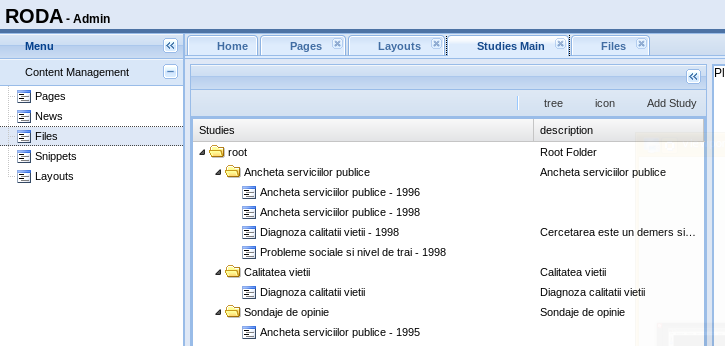
\includegraphics[width=12cm]{img/content-tabs}

\section{Extensii ale sistemului EXTJS pentru interfata de administrare a RODA}

Extensiile sistemului ExtJS sunt extensii ale unor componente standard ale bibliotecii care nu fac parte din namespace-ul RODAdmin (vor fi apelate de componente ale acestuia). 

\subsection{Integrarea editorului CodeMirror}

Editorul CodeMirror este un editor Javascript care permite afisarea diferitelor tipuri de cod (elemente de limbaj de programare) intr-un mod usor de urmarit (cu colorarea diferita a cuvintelor rezervate, numararea liniilor de cod, etc.). Submodulul CMS al aplicatiei RODA are nevoie de un astfel de editor pentru a prezenta fragmentele de cod HTML sau CSS editate. Pentru aceasta a fost necesara extinderea sistemului de layout al campului formularelor 'Ext.layout.component.field.Field' si definirea unui nou tip de camp de formular, special pentru incarcarea editorului CodeMirror. Extinderea componentelor se bazeaza pe o serie de clase definite de Adrian Teodorescu (ateodorescu@gmail.com; http://www.mzsolutions.eu) si publicate in licenta MIT care permite redistribuirea elementelor modificate. 

Pentru utilizarea unui camp de tip codemirror este necesara includerea fisierelor editorului CodeMirror alaturi de fisierele aplicatiei principale si apoi, campul se adauga in formularul respectiv folosind codul urmator: 

\begin{lstlisting}[language=json,firstnumber=1]
    items : [
    	         {
        	         xtype : 'codemirror',
          			 mode : 'htmlmixed',
	                 readOnly : true,
	                 enableFixedGutter : true,
	                 showAutoIndent : false,
	                 showLineNumbers : false,
	                 enableGutter : true,
	                 showModes : false,
	                 pathModes : 'CodeMirror-2.02/mode',
	                 pathExtensions : 'CodeMirror-2.02/lib/util',
	             }
             ]
\end{lstlisting}


\subsection{TreeCombo}

Pentru a putea selecta elemente care se afla intr-o structura arborescenta intr-un component de tip drop-down a fost nevoie de extinderea clasei 'Ext.form.field.Picker'. Componentul TreeCombo este necesar in formularele de introducere (sau de modificare) a intrebarilor studiilor, acolo unde se pot alege concepte cu care acestea pot fi asociate. Conceptele sunt introduse intr-o structura arborescenta. Noul component construieste un panou suplimentar in care integreaza un treeview pe care defineste un eveniment special care transfera elementul selectat catre campul de baza. Prin extinderea elementului Picker si nu a intregului camp (elementul Picker fiind de fapt sageata care determina expandarea campului de baza), odata executata selectia se poate reveni la un camp clasic de formular care va fi trimis catre server corect. 

Apelarea elementului de tip treecombo in formular se face conform codului urmator:

\begin{lstlisting}[language=json,firstnumber=1]
{
	xtype : 'treecombo',
	selectChildren : false,
	fieldLabel : 'Concept',
	store : 'studies.CBEditor.ConceptsDisp',
	itemId : 'conceptselector',
	name : 'concept_id',
	displayField : 'text',
	valueField : 'id',
	canSelectFolders : true,
	itemTreeClick : function(view, record, item,
							index, e, eOpts, treeCombo) {
							var id = record.data.id;
							treeCombo.setValue(id);
	this.collapse();
}


\end{lstlisting}

Iar rezultatul se poate vedea in cele ce urmeaza:

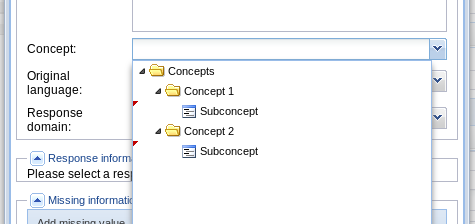
\includegraphics[width=12cm]{img/treecombo}


\section{Procedura de initializare a aplicatiei}

Initializarea aplicatiei se face in functia “launch” din controllerul principal. Etapele sunt prezentate in figura urmatoare.


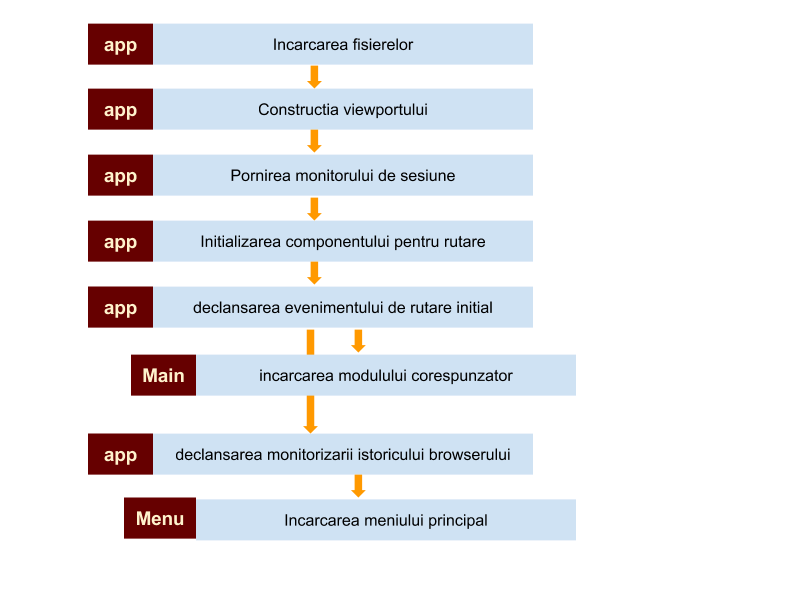
\includegraphics[width=10cm]{img/app-launch}

Dupa finalizarea incarcarii fisierelor de catre componentul de incarcare dinamica, se construieste viewportul principal. Acesta ocupa tot spatiul disponibil in browser si in momentul in care este construit ExtJS ii calculeaza automat dimensiunile pe care le are in acel moment. Constructia viewportului este precedata de citirea unei liste de setari generale de pe server. Dupa constructia viewportului, este pornit monitorul de sesiune care urmareste perioade de inactivitate in interfata mai mari decat un anumit parametru. Monitorul de sesiune trebuie pornit cat mai repede pentru a nu se declansa prea tarziu, in cazul in care faza de initializare a aplicatiei dinainte de pornirea sa dureaza prea mult. 

Dupa pornirea monitorului de sesiune aplicatia trebuie sa vada daca va prezenta viewportul asa cum se incarca el in mod normal sau daca in url-ul apelat exista specificari care necesita apelarea unui anumit submodul care sa se incarce automat. Aceasta se face prin initializarea componentului de rutare. Acesta descompune url-ul initial in functie de separatorul specificat (in cazul nostru \#) si daca este cazul (adica daca exista un \# in url si este urmat de o succesiune de caractere) declanseaza un eveniment care va fi preluat de controllerul principal ('RODAdmin.controller.Main'). In cazul in care sirul de caractere de dupa \# din url contine o instructiune valida, controllerul principal va incarca submodulul corespunzator. 

Dupa verificarea modului de initializare, se declanseaza monitorizarea istoricului browserului care va declansa acelasi eveniment (numit tokenchange) de cate ori se modifica acesta. Pe toata durata rularii aplicatiei, daca istoricul se modifica, controllerul principal va reactiona in functie de ce se specifica dupa caracterul . 

Dupa toate aceste pregatiri, se solicita de la server incarcarea store-ului cu continutul adaptat al meniului in functie de drepturile utilizatorului curent. Dupa obtinerea datelor, se incarca meniul principal de catre controllerul 'RODAdmin.controller.Menu'. 

\section{Module ale interfetei}

\subsection{Dashboard}

\subsubsection{Prezentare si arhitectura}

Modulul dashboard este primul care se afiseaza, in cazul in care nu exista o solicitare suplimentara facuta prin sistemul de rutare. Chiar daca exista o astfel de solicitare, modulul Dashboard se incarca oricum si va fi disponibil in tab-ul Home.

Arhitectura acestui modul este putin diferita de arhitectura altor module. Majoritatea modulelor interfetei de administrare RODA sunt concepute sa permita afisarea si administrarea unui singur element (fie ca este vorba despre fisiere, studii, etc). Modulul Dashboard (ca si modulul Metadata prezentat mai jos) este diferit prin aceea ca trebuie sa permita prezentarea mai multor elemente concomitent. Acestea trebuie sa poata fi rearanjate, daca se doreste aceasta si minimizate in cazul in care operatorul doreste sa se concentreze asupra unuia dintre ele. 

Dashboardul este impartit in doua coloane, fiecare coloana putand contine oricate componente, numite “portlet”. Deocamdata exista patru astfel de componente dar adaugarea de componente noi este relativ simpla. 

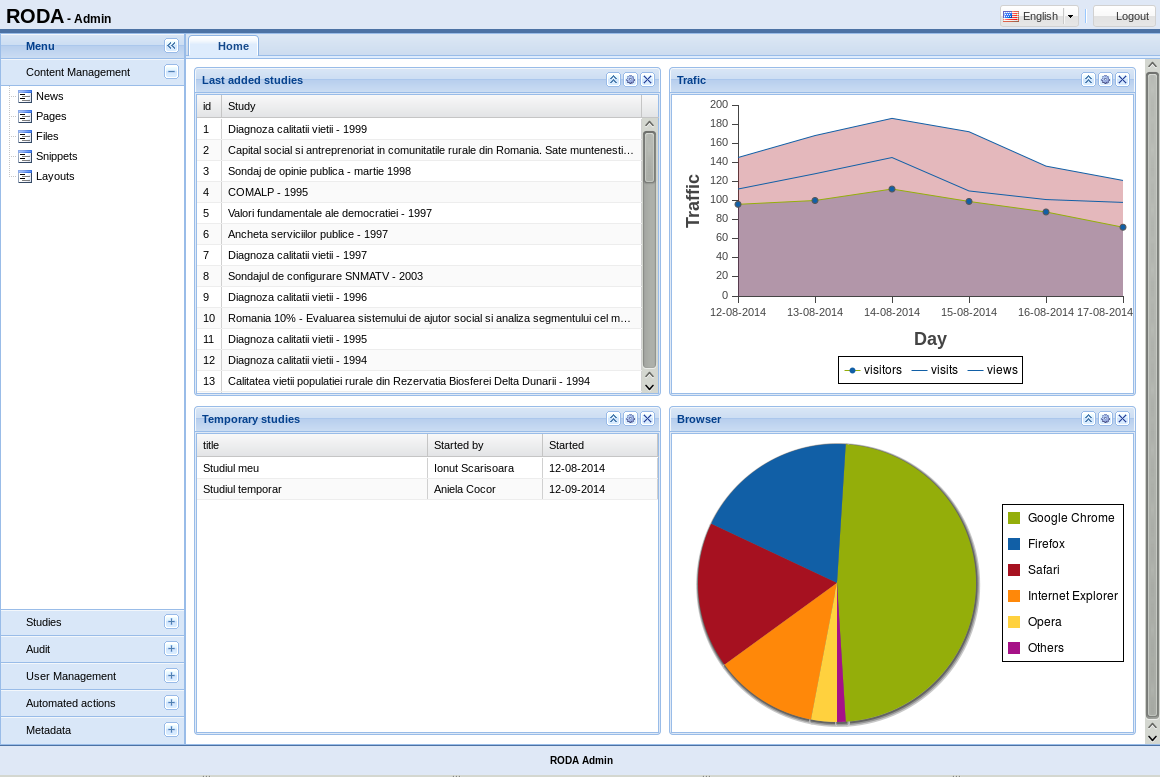
\includegraphics[width=16cm]{img/dashboard}

Dashboardul este implementat pornind de la o clasa principala, numita 'RODAdmin.view.dashboard.Dashboard' care are alias-ul "dashboard" si care este cea apelata in momentul incarcarii. Clasa Dashboard extinde o clasa numita 'RODAdmin.view.dashboard.DashboardPanel', care la randul ei este o extensie a clasei 'Ext.panel.Panel' care face parte din biblioteca ExtJS. Motivul pentru care a fost necesara extinderea clasei 'Ext.panel.Panel' este nevoia de a adauga o serie de verificari si operatiuni care trebuie sa se execute la initilizarea componentului si inainte de executia layoutului acestuia (constructia elementelor de afisare). De asemenea, 'RODAdmin.view.dashboard.DashboardPanel' inregistreaza o zona speciala numita 'RODAdmin.view.dashboard.DashboardDropZone' care permite apoi mutarea componentelor dintr-o coloana in alta. 

In clasa 'RODAdmin.view.dashboard.Dashboard' sunt inregistrate doua coloane, in fiecare coloana fiind incarcate unul sau mai multe componente care pot contine orice fel de elemente de interfata ExtJS. 

\subsubsection{Componentele dashboardului}

\textbf{Ultimele studii adaugate} Un component tabelar care afiseaza ultimele studii adaugate in baza de date. 
\textbf{Trafic} Un grafic al traficului pe pagina www.roda.ro
\textbf{Studii temporare} Un tabel al studiilor aflate in curs de editare
\textbf{Browsere} O statistica a browserelor cu care a fost accesat site-ul www.roda.ro. 


\section {Modulul de management al metadatelor}

Modulul de management al metadatelor este conceput si implementat pentru datele suport care nu au nevoie de o interfata complexa pentru intretinere. Asemanator ca implementare cu dashboardul (ecranele se pot muta de pe o coloana pe alta si se pot minimiza in functie de nevoi) modulul de metadate este de asemenea usor extensibil pentru a permite adaugarea de noi componente in functie de necesitati. In imaginea urmatoare se pot vedea deschise modulele pentru modificarea prefixelor si a sufixelor personale precum si cel de orase / localitati.

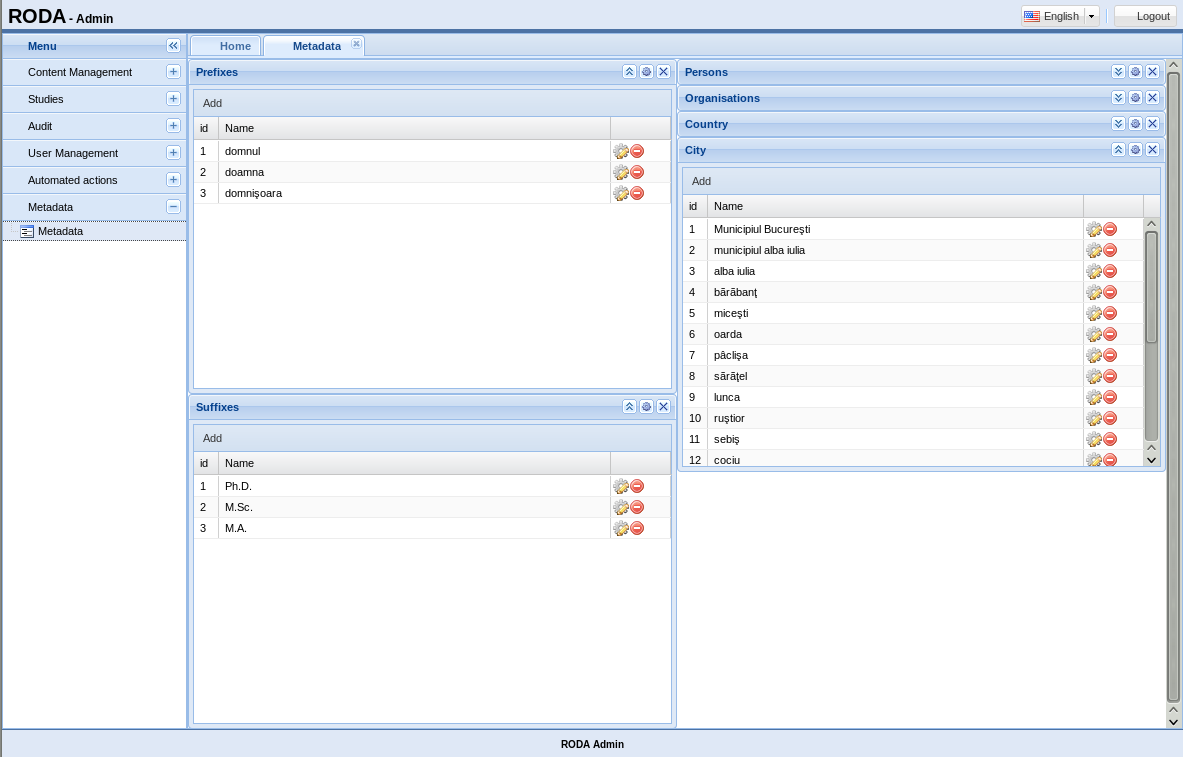
\includegraphics[width=16cm]{img/metadata}

Celelalte componente (persoane, organizatii, tari) sunt inchise pentru a nu mai ocupa spatiu pe ecran. Fiecare component al modulului permite operatii elementare de adaugare, modificare si/sau stergere in masura in care este cazul.

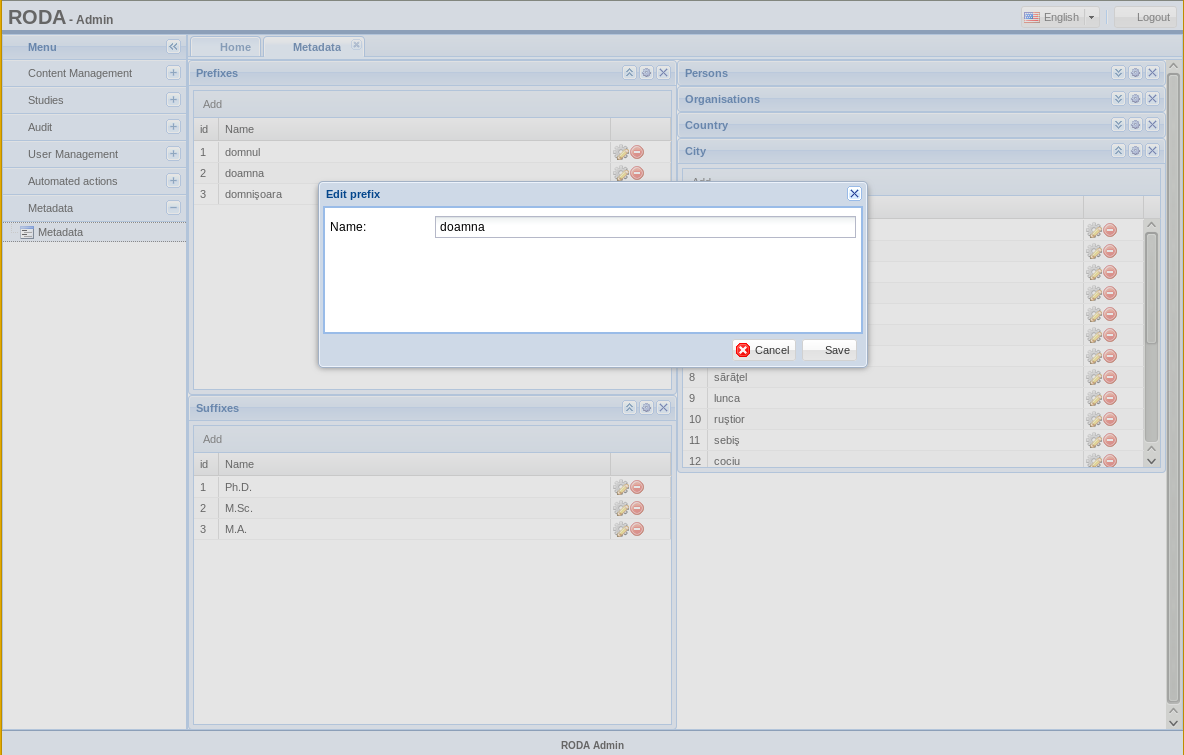
\includegraphics[width=16cm]{img/metadata-form}


\section {Modulul de management al continutului}

Acest modul a fost prezentat pe larg intr-un raport anterior. Pentru coerenta, reluam aici elementele sale in mod succint:

\textbf{Layout} submodul de management al layouturilor. Layouturile sunt elemente HTML care compun tot ceea ce defineste o pagina WEB, mai putin continutul textual al acesteia (header, footer, meniuri, coloane laterale, etc.). Submodulul layout permite afisarea arborescenta sau liniara a layouturilor disponibile, adaugarea de noi layouturi si modificarea celor existente.

\textbf{Snippet} submodul care permite modificarea, urmarirea si introducerea de fragmente de cod care pot fi integrate apoi in alte componente CMS. 

\textbf{Pagini} submodul care permite urmarirea, afisarea si modificarea paginilor care compun aplicatia RODA. De aici se poate modifica continutul paginilor, se pot modifica layouturile acestora precum si ierarhia lor.
\textbf{Fisiere} submodulul dedicat fisierelor, conectat direct cu un sistem de repository bazat pe Apache Jackrabbit™ content repository permite vizualizarea, adaugarea, modificarea si stergerea de fisiere (imagini, documente, etc.).


\section {Modulul de management al utilizatorilor}

De asemenea prezentat intr-o alta faza a proiectului, modulul de management al utilizatorilor permite vizualizarea, adaugarea, urmarirea utilizatorilor RODA si a activitatii acestora. 


\section {Modulul de management al studiilor}

Modulul de management al studiilor este cel mai complex modul din interfata de administrare RODA  si este conceput pentru a permite toate operatiile necesare cu studiile care se gasesc in arhiva RODA. Modulul are trei componente principale: 
    - Componentul de vizualizare a studiilor existente
    - Editorul principal
    - Editorul DDI. 

\subsection{Componentul de vizualizare a studiilor existente}

Componentul de vizualizare permite urmarirea tuturor studiilor si a elementelor acestora. Componentul imparte ecranul in doua suprafete distincte, una care contine lista studiilor, prezentata fie ca arbore de cataloage, fie ca lista simpla. Respectand aceeasi paradigma vizuala pe care o folosim in toata aplicatia RODA, la selectarea unui studiu din lista din panoul stang, in panoul din partea dreapta si afiseaza detaliile studiului. 

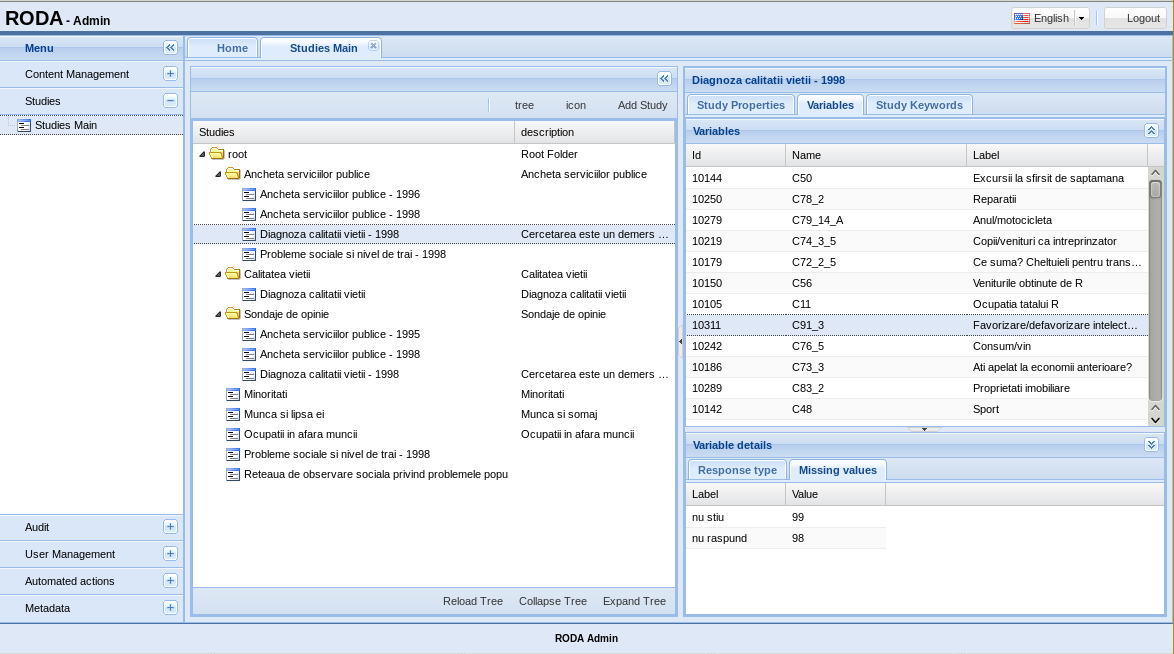
\includegraphics[width=16cm]{img/study-tree-compl}

Panoul de vizualizare a unui studiu este impartit in mai multe tab-uri, in functie de complexitatea structurii de date. Aceste taburi apar doar in masura in care studiul curent contine date pentru afisarea lui. 
 
\textbf{Proprietati} - acest tab afiseaza titlu, descriere, alte elemente descriptive cum ar fi universul, ponderarile (daca este cazul), acoperirea geografica, etc. 

\textbf{Institutii/Persoane} - acest tab afiseaza institutiile si persoanele implicate in realizarea sau finantarea acestui studiu. O institutie (sau o persoana) poate juca mai multe roluri in realizarea unui studiu, poate fi finantator, poate fi realizator al chestionarului

\textbf{Date/Intervale} - tabul afiseaza datele sau intervalele de timp in care s-au intamplat diferite activitati ale studiului. Standardele curente     permit specificarea diferitelor momente in executia unui studiu (proiectarea chestionarului, colectarea datelor, etc.)

\textbf{Variabile} - lista de variabile asociate studiului impreuna cu elementele definitorii ale acestora (tipul de raspuns, valorile lipsa, etc.). 

\textbf{Cuvinte cheie} - Lista cuvintelor cheie asociate studiului respectiv. 


\subsection{Editorul principal}

Editorul principal permite modificarea proprietatilor studiilor existente. Editorul principal este structurat conform standardelor de reprezentare a datelor sociale propuse de DDI (Data Documentation Initiative). Noile versiuni ale formatului DDI (incepand de la versiunea 3.0 in sus) sunt concepute astfel incat sa capteze in mod distinct toate etapele dezvoltarii unui studiu (lifecycle). Ca si interfata de vizualizare, editorul este impartit in mai multe tab-uri, cu diferenta ca aici toate sunt vizibile indiferent de prezenta continutului. 

Editorul principal este diferit de celelalte componente ale interfetei descrise pana acum prin aceea ca fiecare studiu in curs de editare se deschide intr-un tab principal al aplicatiei, la acelasi nivel cu modulele aplicatiei, pentru a putea avea la dispozitie toata suprafata panoului principal pentru editarea studiului. 

Editorul este impartit in 6 componente:

\subsubsection{Study proposal}

In panoul study proposal sunt disponibile toate elementele care in mod normal se completeaza in faza de proiectare a studiului. 

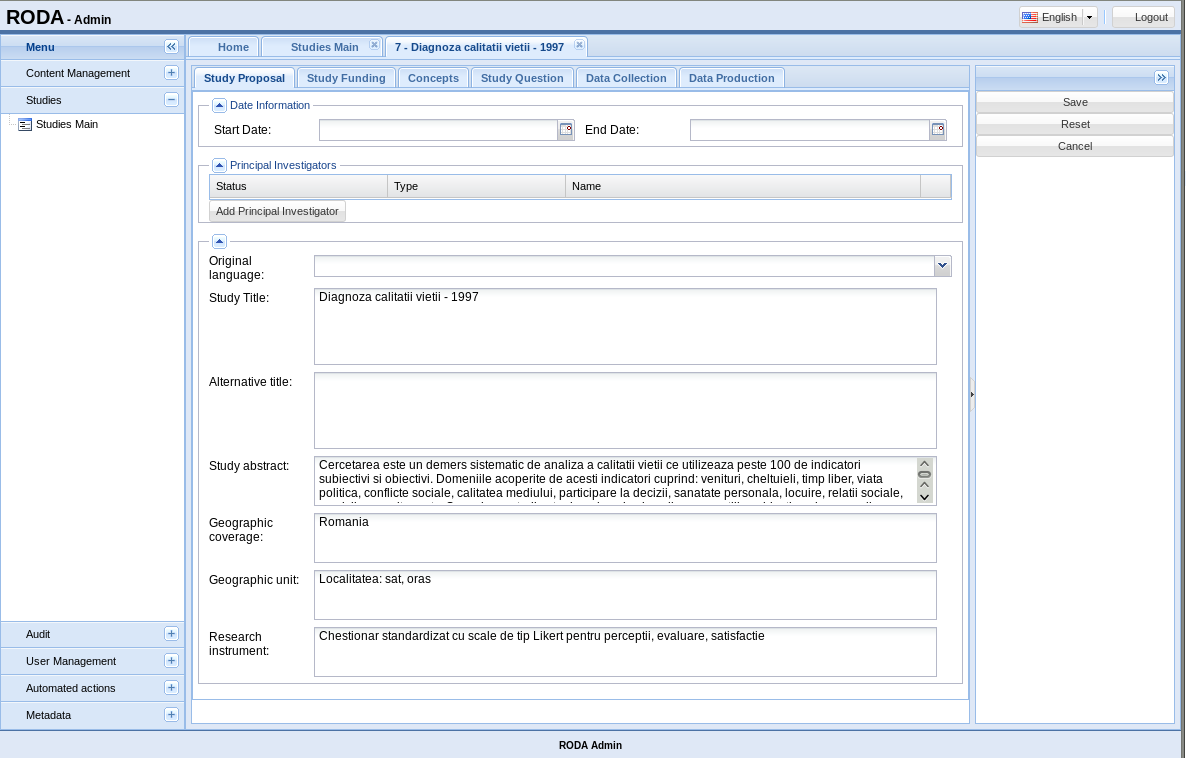
\includegraphics[width=16cm]{img/studyedit-proposal}


In panoul “Study Funding” sunt afisate elementele care tin de finantarea studiului respectiv, in masura in care sunt cunoscute:

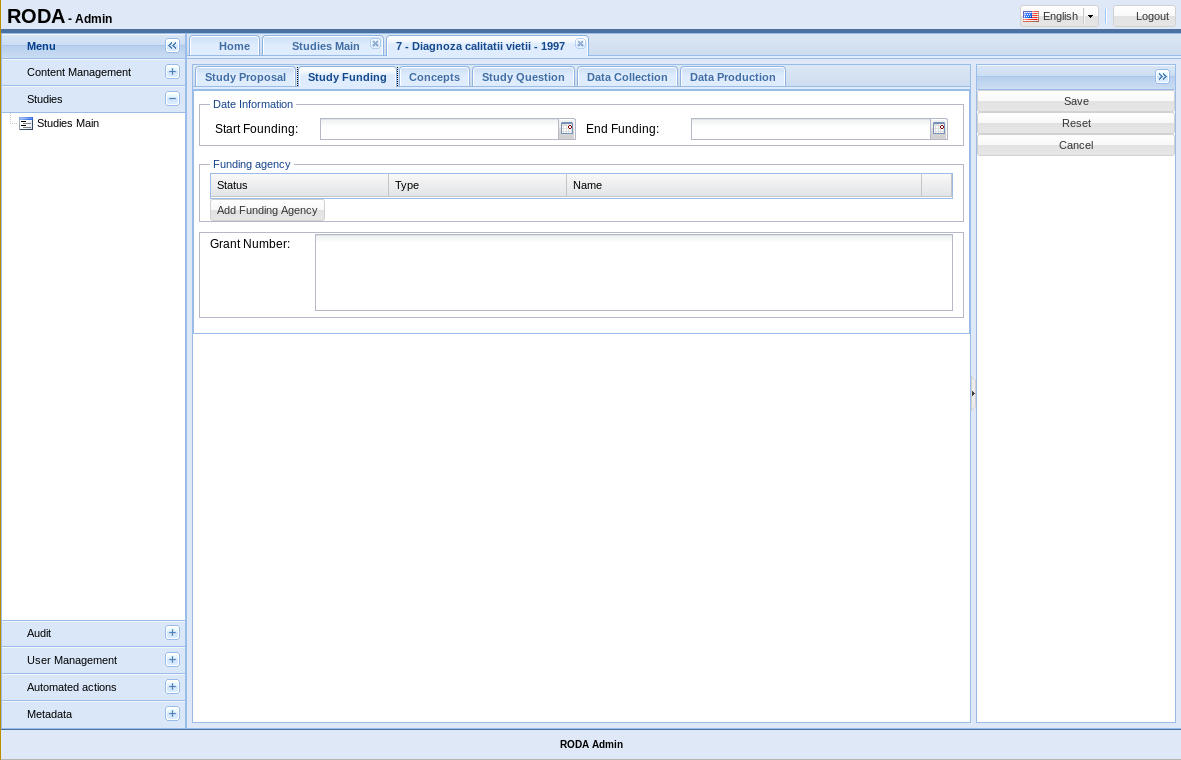
\includegraphics[width=16cm]{img/studyedit-funding}

Conceptele permit gruparea intrebarilor in functie de semnificatii mai abstracte. In esenta, la nivelul datelor, conceptele sunt grupuri de intrebari distribuite intr-o structura arborescenta. Panoul de concepte contine informatiile despre conceptele studiului curent, in masura in care acestea sunt disponibile.

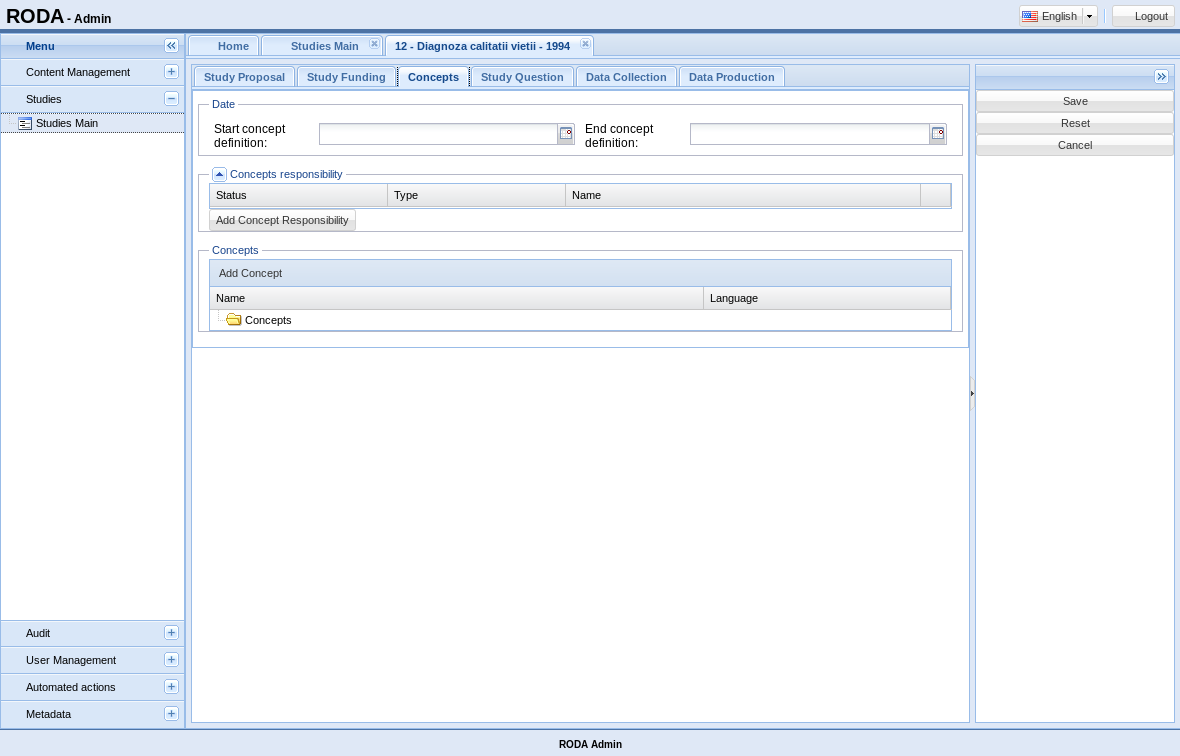
\includegraphics[width=16cm]{img/studyedit-concepts}

Panoul de intrebari este panoul in care se pot modifica/introduce intrebarile studiului, impreuna cu traducerile acestora si persoanele sau organizatiile responsabile de alcatuirea chestionarului. 

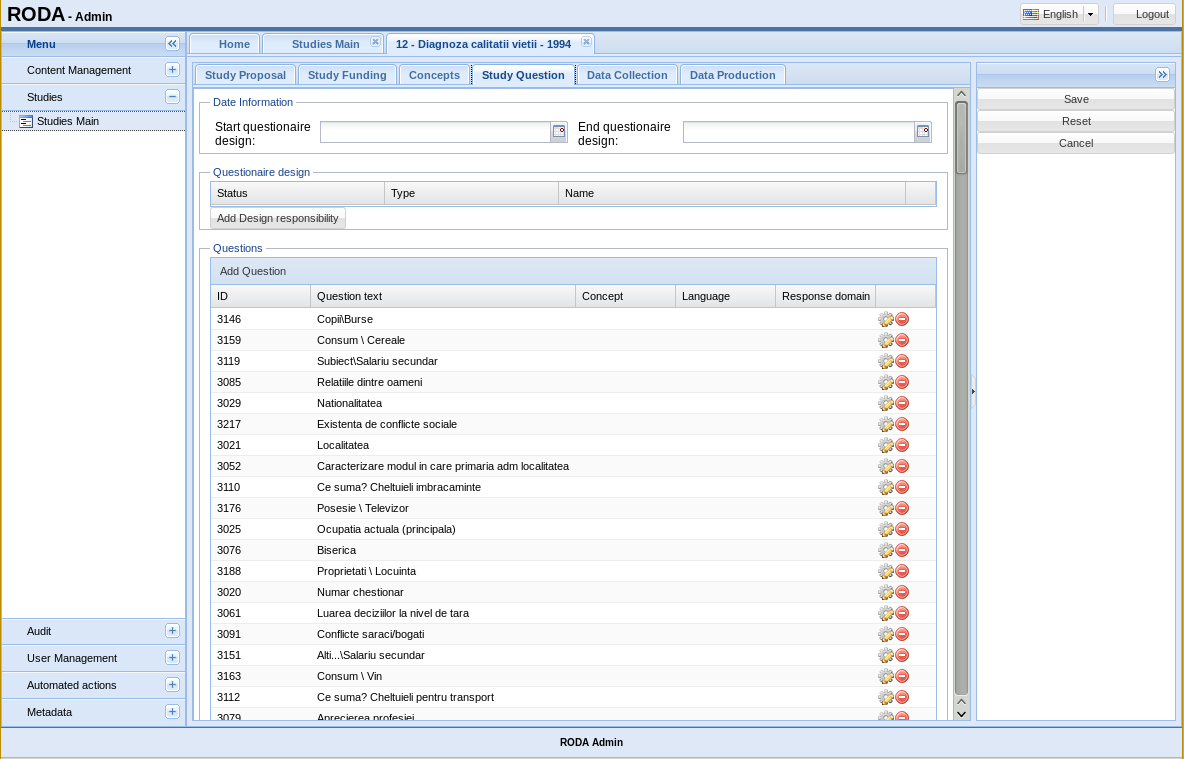
\includegraphics[width=16cm]{img/studyedit-questions}

Panoul Data Collection contine informatii despre procesul de colectare a datelor, perioadele in care acestea au avut loc, impreuna cu persoanele sau organizatiile responsabile, modul de colectare (interviu fata in fata, telefonic, etc). 

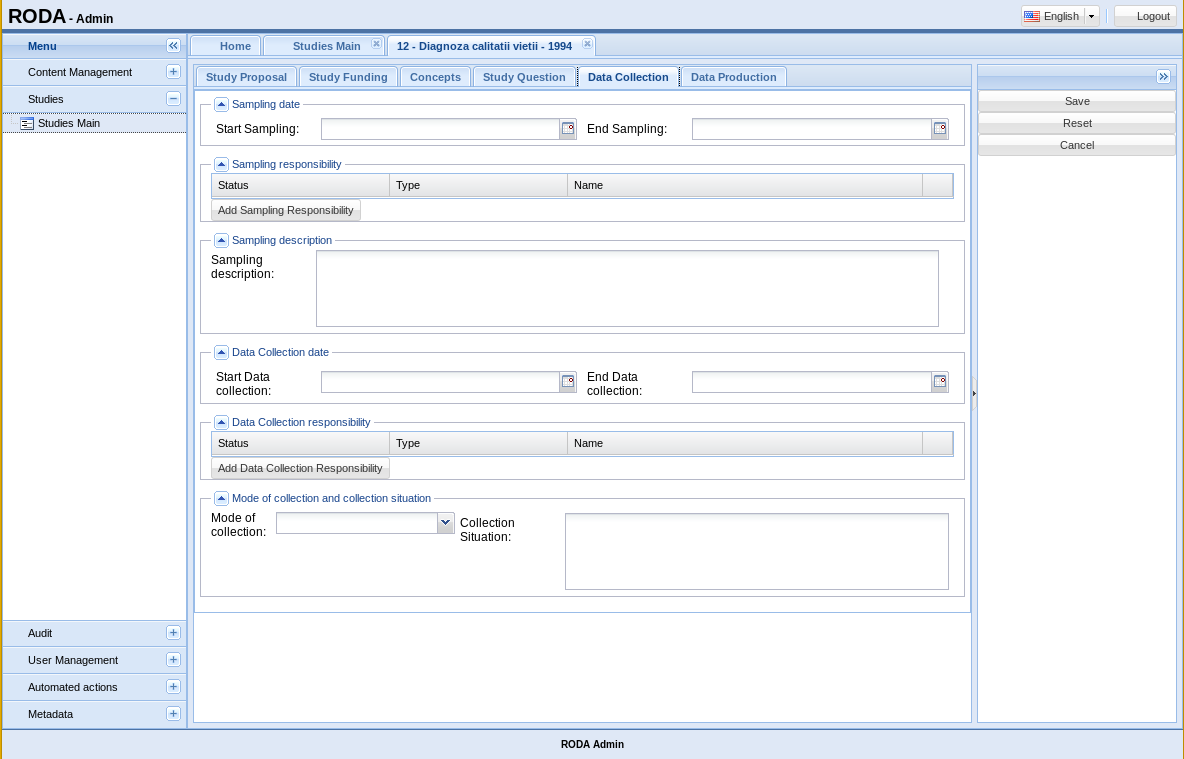
\includegraphics[width=16cm]{img/studyedit-datacollection}

Panoul “DataProduction” este cel in care se gasesc informatii depre variabile. 

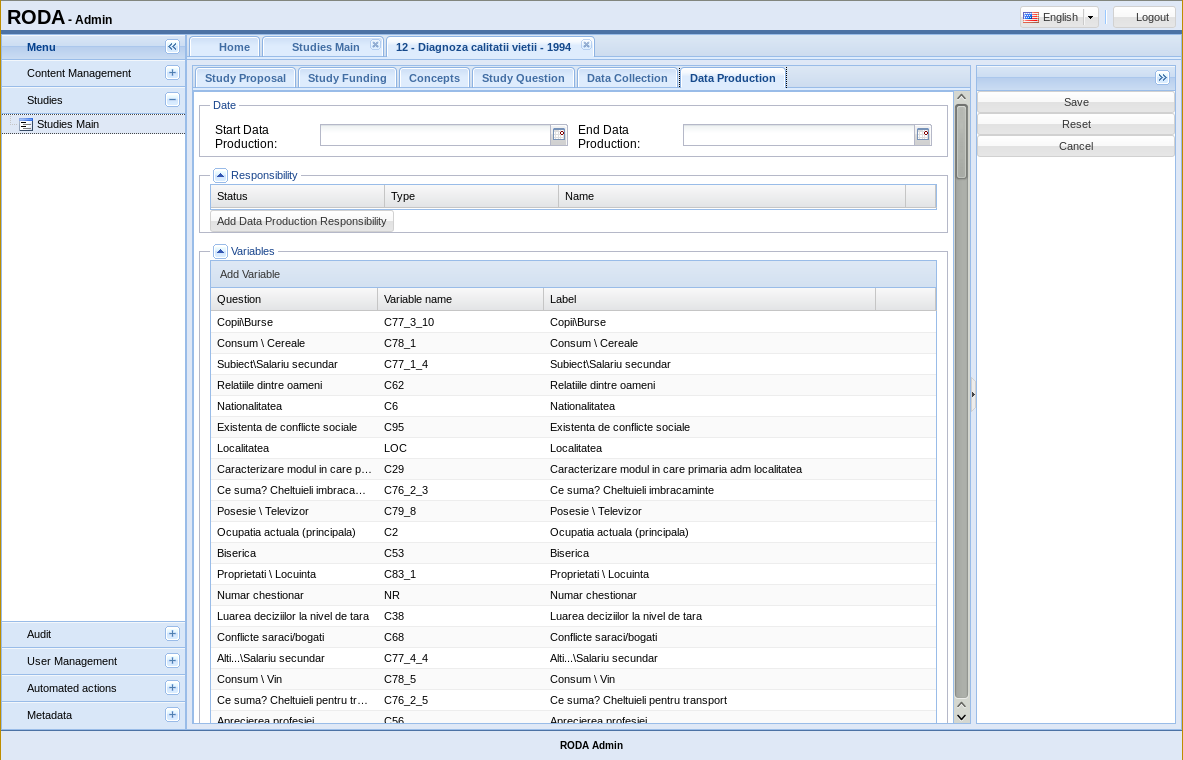
\includegraphics[width=16cm]{img/studyedit-dataproduction}


\subsection{Editorul DDI}


Editorul DDI este un set de formulare asemanatoare cu cele care alcatuiesc componentul de editare a studiului. Editorul DDI insa este complet separat de structura principala a bazei de date si este conceput pentru cazurile in care un operator RODA sau un utilizator extern doreste sa introduca un studiu in baza de date sau sa creeze un fisier in format DDI. Toate componentele editorului DDI sunt separate de cele ale formularelor de editare a studiilor, inclusiv componentele de tip store si model. 

Datele completate in editorul DDI sunt salvate pe server periodic pentru a nu se pierde in cazul in care operatorul face o pauza sau se intrerupe conexiunea cu serverul. Datele sunt inregistrate intr-o sectiune speciala a serverului intr-o forma compacta si raman disponibile putand fi reincarcate in editorul DDI de cate ori este nevoie. 

La finalizarea procesului de editare, operatorul poate semnala sistemului ca doreste ca studiul sa fie integrat in arhiva RODA. Sistemul va aplica o serie de validari asupra datelor si, daca verificarile determina faptul ca datele sunt corecte, studiul este introdus in baza de date si este sters din sistemul de stocare temporar. 

Editorul DDI poate fi utilizat si pentru editarea fisierelor existente in format DDI. Formatul fiind foarte extins, editorul va extrage din fisier doar componentele pe care le cunoaste. In cazul in care documentul va fi inregistrat in arhiva RODA, in baza de date a serverului se vor inregistra doar elementele pe care editorul se poate citi, celelalte ramanand in fisierul XML. 

Componentele editorului DDI sunt modelate dupa acelasi sistem de inregistrare a evolutiei studiului (lifecycle) pe care il propune formatul DDI incepand cu versiunea 3.0 ca si editorul studiilor din baza de date. 

Study Proposal - elementele care in mod normal se completeaza in faza de proiectare a studiului, in principiu perioada (sau data) initierii studiului, persoanele sau organizatiile responsabile pentru propunerea studiului, limba principala precum si elementele descriptive principale ale studiului (abstract, titlu, unitatea de analiza, etc.). Data initierii studiului, in functie de cat de multe se stiu despre aceasta faza, poate fi o singura data sau un interval.


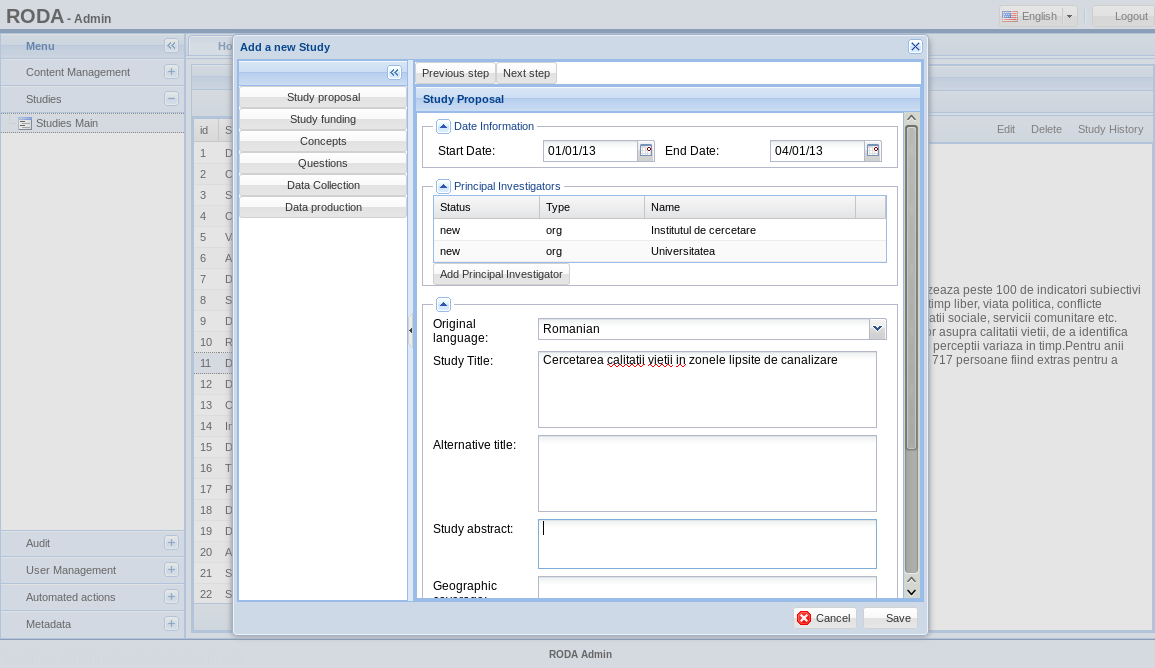
\includegraphics[width=16cm]{img/ddi-editor-proposal}

Panoul “Study Funding” se ocupa de procesul de finantare a studiului. Aici vor trebui introduse organizatiile si/sau persoanele responsabile de finantarea studiului precum si perioada in care finantarea a fost disponibila. Exista posibilitatea introducerii numarului grantului (sau codului grantului).


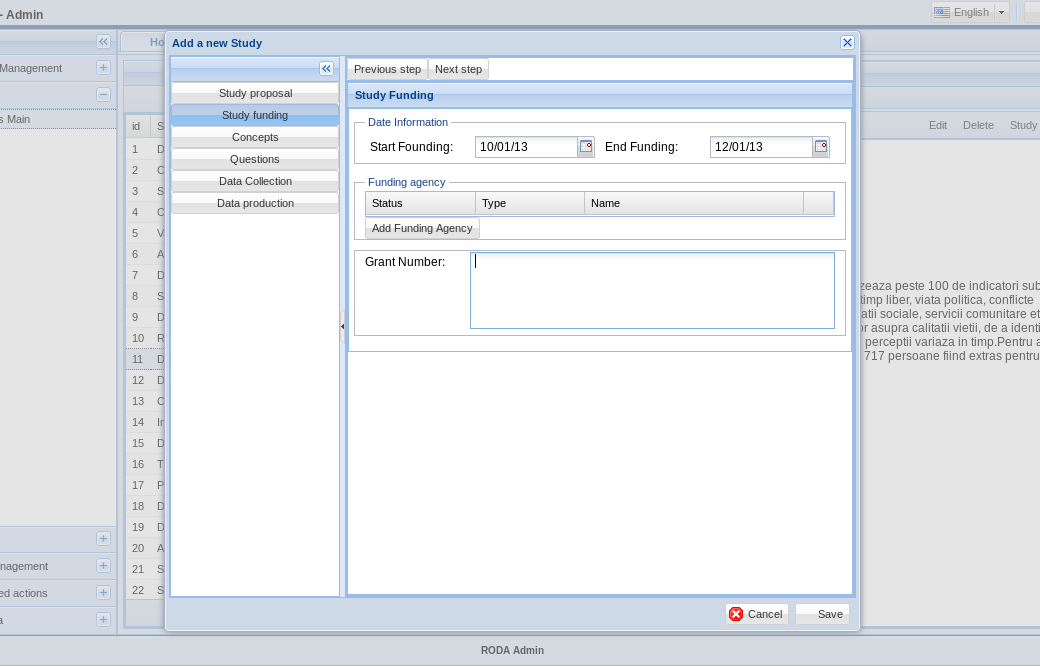
\includegraphics[width=16cm]{img/ddi-editor-funding}


DDI defineste conceptele ca fiind grupuri de intrebari. Un studiu poate fi introdus in baza de date si specificat in DDI fara concepte, ele nu sunt in nici un fel obligatorii. De asemenea, anumite intrebari pot fi grupate in concepte in timp ce altele pot samane in afara acestora. Oricum ar fi, in situatia in care studiul are intrebarile grupate in concepte, in acest panou pot fi specificate. 


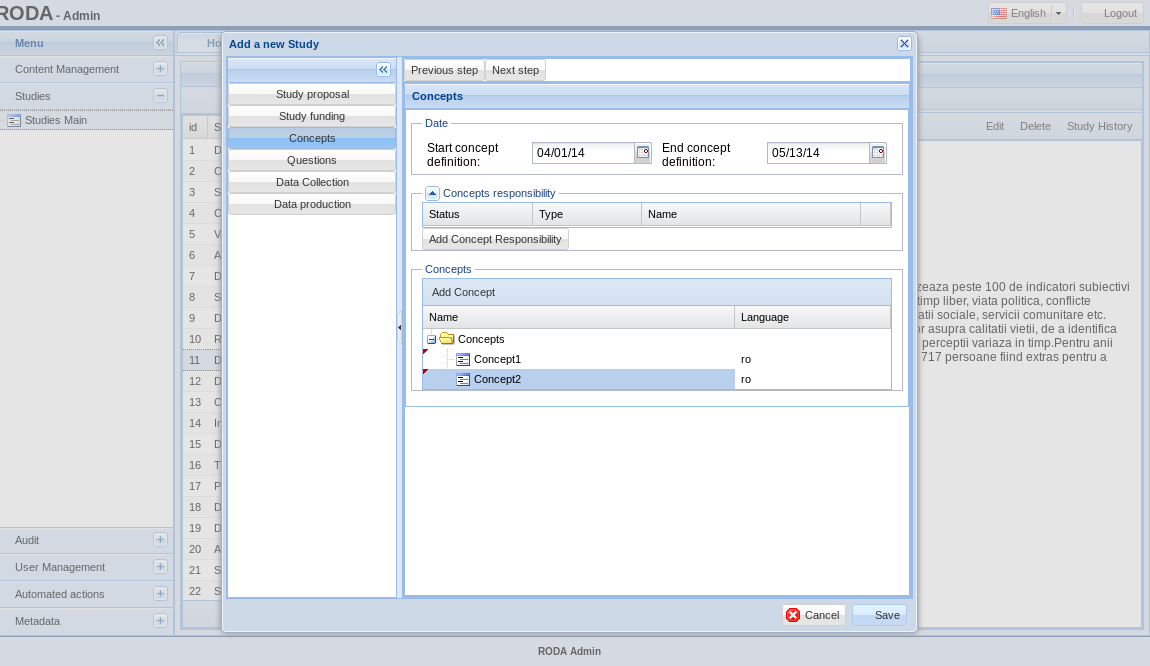
\includegraphics[width=16cm]{img/ddi-editor-concepts}


In panoul cu intrebarile se vor introduce intrebarile din chestionar, impreuna cu variantele de raspuns posibile si cu codificarea valorilor lipsa. In figura urmatoare se observa panoul de introducere a unei intrebari al carui tip de raspuns este numeric. 

Tot in acest panou este posibila traducerea intrebarilor (in cazul in care este nevoie). Pentru fiecare intrebare se pot introduce mai multe traduceri in limbi diferite. Este posibila de asemenea traducerea categoriilor de raspuns si valorile lipsa. 

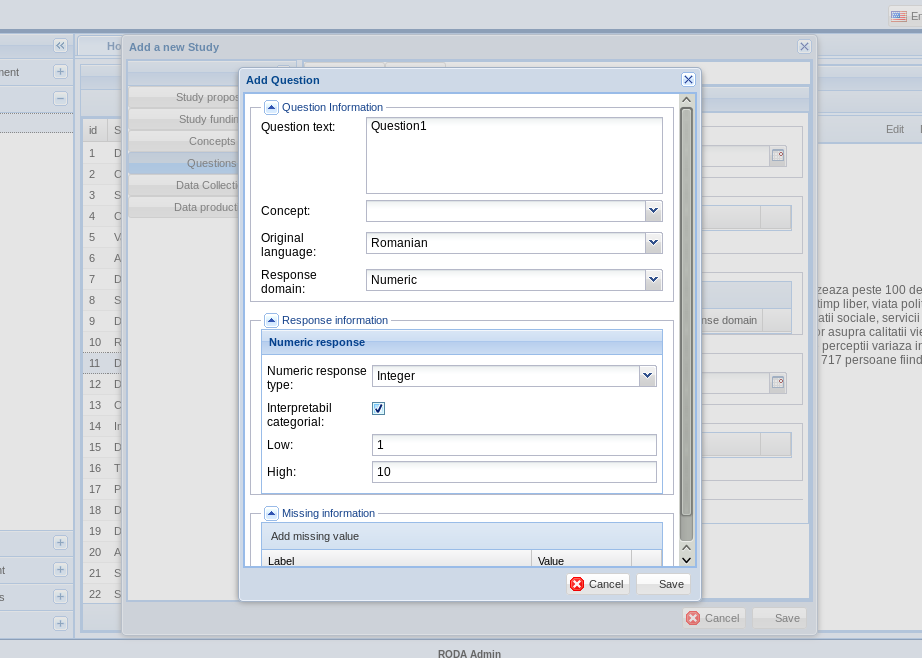
\includegraphics[width=16cm]{img/ddi-editor-addquestion}


Data Collection contine informatii despre procesul de colectare a datelor, fiind posibile specificarea persoanelor sau organizatiilor responsabile de colectarea datelor, specificarea modului de colectare (interviuri directe, interviuri telefonice, e-mail, etc.).

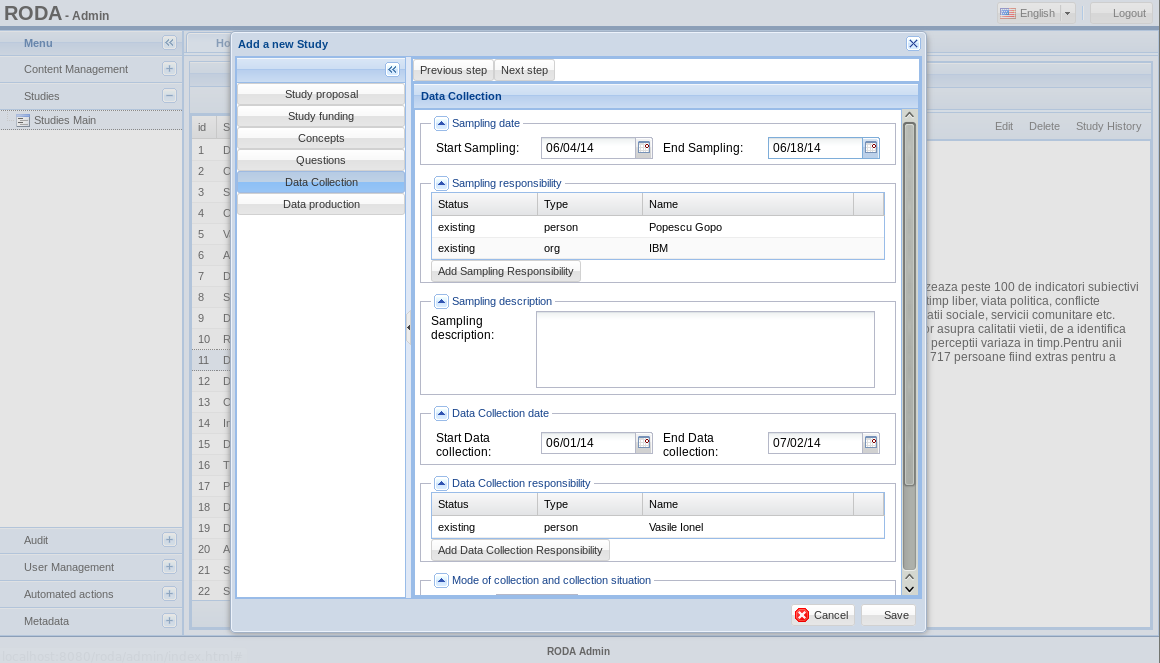
\includegraphics[width=16cm]{img/ddi-editor-datacollection}

Ultimul panou, cel numit “data production” este cel in care trebuiesc introduse variabilele. In standartul DDI o intrebare poate fi reprezentata cu ajutorul mai multor variabile. Fiecare variabila va mosteni tipul de raspuns si lista de codificari specificare la intrebare. 

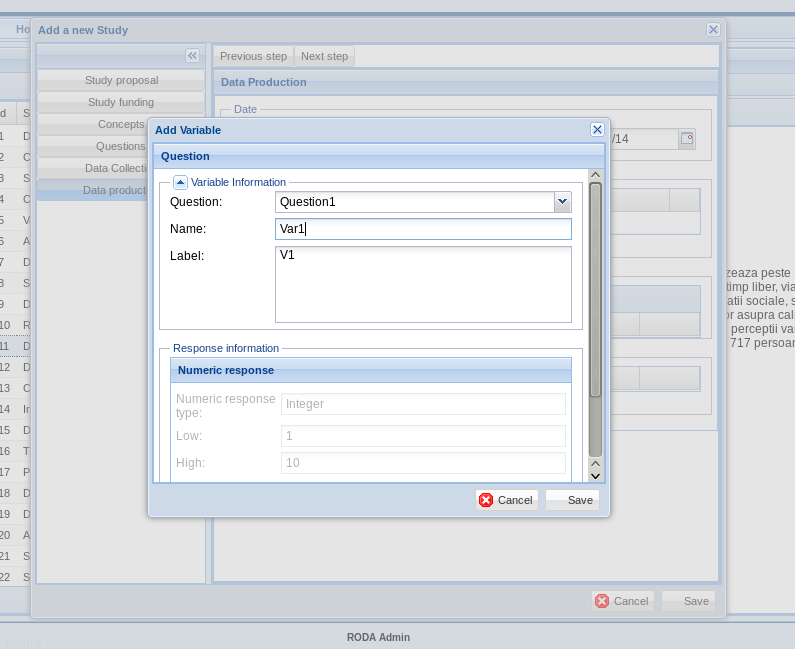
\includegraphics[width=16cm]{img/ddi-editor-addvariable}
